%!TEX TS-program = xelatex
%!TEX encoding = UTF-8 Unicode

\documentclass[12pt]{extarticle}
% extarticle is like article but can handle 8pt, 9pt, 10pt, 11pt, 12pt, 14pt, 17pt, and 20pt text

\def \ititle {Origins of Mind}

\def \isubtitle {Lecture 01}

\def \iauthor {Stephen A. Butterfill}
\def \iemail{s.butterfill@warwick.ac.uk}
\date{}

%for strikethrough
\usepackage[normalem]{ulem}

\input{$HOME/Documents/submissions/preamble_steve_handout}

%\bibpunct{}{}{,}{s}{}{,}  %use superscript TICS style bib
%remove hanging indent for TICS style bib
%TODO doesnt work
\setlength{\bibhang}{0em}
%\setlength{\bibsep}{0.5em}


%itemize bullet should be dash
\renewcommand{\labelitemi}{$-$}

\begin{document}

\begin{multicols*}{3}

\setlength\footnotesep{1em}


\bibliographystyle{newapa} %apalike

%\maketitle
%\tableofcontents




%---------------
%--- start paste






\def \ititle {Lecture 01: Seeing Red: Do Humans Visually Experience Categorical Colour Properties?}

\begin{center}

{\Large

\textbf{\ititle}

}



\iemail %

\end{center}



\section{A ‘subject-determining platitude’ about colour}

‘If someone with normal color vision looks at a tomato in good light, the tomato will appear to have a distinctive property—a property that strawberries and cherries also appear to have, and which we call ‘red’ in English’ \citep[p.\ 4]{byrne:2003_color}

It is a ‘subject-determining platitude’
that ‘“red” denotes the property of an object putatively presented in visual experience
when that object looks red’, and likewise for other colour terms
\citep[pp.\ 199--200]{Jackson:1996zz}.

Question:
Does ‘“red” denote the property of an object putatively presented in visual experience when that object looks red’?


Simplifying assumptions:



1. There is a property denoted by ‘red’ which some objects have;  call this property   \emph{red}.


2. If the property \emph{red} (say) is presented in visual experience, then things which have this property  thereby differ in  visual appearance from things which do not have it.


Question (reformulated):
Do red things differ in visual appearance from non-red things?




\section{Do you visually experience red because you call things ‘red’?}

“surprising it would be indeed if I have a perceptual experience as of red because I call the perceived object ‘red’.”
\citep[pp.~324--5]{Stokes:2006fd}.

Argument:
\begin{enumerate}
\item Red things differ in visual appearance from non-red things.
\item The capacity to detect the difference in visual appearance between
red and non-red things is, or depends on, the capacity to visually
discriminate red and non-red things.
\item The capacity to visually discriminate red and non-red things depends
on the capacity to label the red things (for example, using ‘red’).
\end{enumerate}
Therefore:
\begin{enumerate}[resume]
\item I have a perceptual experience as of red span.italic
because span I call the perceived object ‘red’.
\end{enumerate}



\section{How to Measure Phenomenology}

\begin{center}
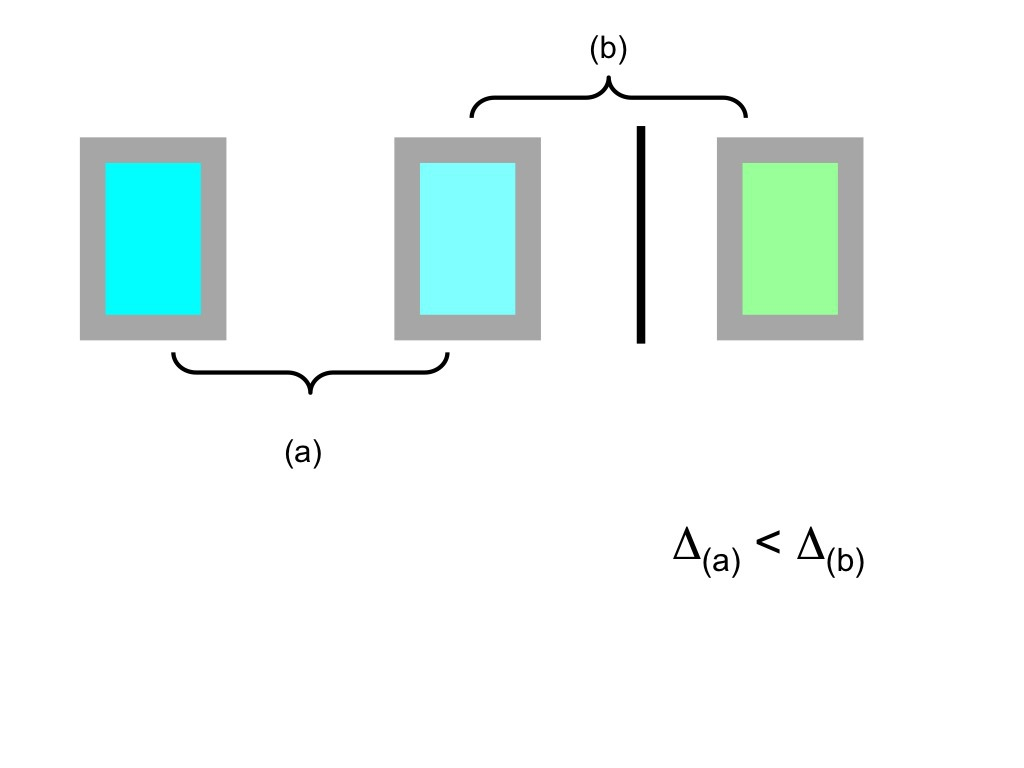
\includegraphics[scale=0.25]{img/categorical_colour_difference3.jpg}
\end{center}
Methods:
\begin{enumerate}

\item People are asked to judge, for each sequence, which of the two outer
things is more similar to the middle thing. Given that visual appearances typically influence
judgements of similarity, if things which differ in whether they are
\emph{red} thereby differ in visual appearance, we would expect people to
judge that the outer thing which is \emph{red} is more similar to the
middle thing than the other outer thing
\citep{kay_what_1984,witzel2014category}.

\item People are asked to the middle object so that it appears to be mid-way
between the two outer objects. (What people are in fact adjusting here is
the hue of the object, but no mention is made of hue: their instructions
are to match differences in appearance.) If things which differ in whether
they are \emph{red} thereby differ in visual appearance, we would expect
people to compensate for this in adjusting hue. In fact they do not
\citep{witzel2014category}.

\item Perceptual grouping: people make visual judgements about orientation which
reveal how things differing in colour are perceptually grouped.  If things which differ in whether
they are \emph{red} thereby differ in visual appearance, we would expect
this to affect how things are perceptually grouped \citet{webster:2012_color}.

\end{enumerate}

The ‘name strategy’: ‘We propose that faced with this situation the
English-speaking subject reasons
unconsciously as follows: “It's hard to decide here which one looks the most
different. Are there any other kinds of clues I might use? Aha! A and B are
both CALLED green while C is CALLED blue. That solves my problem; I'll pick C
as most different.” ... this cognitive strategy ... we will call the
“name strategy”’ \citep[p.~72]{kay_what_1984}.

‘Subjective similarity judgments follow
discrimination distance and reflect no influence from lexical category
boundaries.’ \citep[p.~73]{kay_what_1984}



\section{Why Do Some Claim to Visually Experience Red?}

Suppose, as argued, it is untrue that humans visually experience red or any
other categorical colour properties.
Why have so many philosophers have assumed the opposite, and done so without argument?

Some time after learning to use a colour term like ‘red’
somewhat accurately, humans become faster and more accurate at
distinguishing things which differ in whether they have the property
denoted by that colour term (faster: \citealp{Bornstein:1984cb}; more
accurate: \citealp[p.\ 22--7]{Roberson:1999rk}; not usually immediately:
\citealp{Franklin:2005hp}). In fact, methods highly similar to those which
indicate the absence of appearances do reveal that these properties affect
speed and accuracy of discrimination (\citealp{witzel:2014_categorical}).
As discrimination of these colour properties depends on pre-attentive
processes which are automatic in some of the senses that perceptual
processes are \citep{Daoutis:2006ij,clifford_color_2010}, the abilities to
discriminate may intuitively give rise to the impression that properties
like \emph{red} affect how things appear.





%--- end paste
%---------------

\footnotesize
\bibliography{$HOME/endnote/phd_biblio}

\end{multicols*}

\end{document}
